\documentclass[resume]{subfiles}


\begin{document}
\section{Autres}
\label{sec_autres}
\subsection{Intégration par partie}
$$\int_{a}^{b}u'v=uv\Big|_{a}^{b}-\int_{a}^{b}uv'$$
\subsubsection{exemple}
\begin{align*}
\int_{0}^{1}x^2\cdot sin(n\pi x)dx=\int_{0}^{1} f dg = fg\Big|_{0}^{1} - \int_{0}^{1} g df \\
f=x^2, dg= sin(n\pi x)dx\\
df=2x\cdot dx, g = -\frac{cos(n\pi x)}{n\pi}\\
= -\frac{x^2\cdot cos(n\pi x)}{n\pi}\Big|_{0}^{1}+\int_{0}^{1} \frac{2x\cdot cos(n\pi x)}{n\pi}
\end{align*}

\subsection{Changement de variable}
\subsubsection{Méthode 1}
Lorsque la dérivée $\varphi'(t)$ est présente 
$$\int_{a}^{b}f(\varphi(t))\varphi'(t)dt=\int_{\varphi(a)}^{\varphi(b)}f(x)dx$$
\subsubsection{Méthode 2}
Si $\varphi'(t)=\varphi'=\text{constante}$
$$\int_{a}^{b}f(\varphi(t))dt=\frac{1}{\varphi'}\int_{\varphi(a)}^{\varphi(b)}f(x)dx$$
\subsection{Solutions générales}
\begin{align*}
X''&=-\beta^2 X&&\longrightarrow X(x)=A\cos(\beta x)+B\sin(\beta x)\\
X''&=\beta^2 X&&\longrightarrow X(x)=A\cosh(\beta x)+B\sinh(\beta x)\\
X''&=0 &&\longrightarrow X(x)=Ax+B
\end{align*}

\subsection{Équation d'euler}
$$e^{jx}=\cos(x)+j\sin(x)$$
\subsection{Séparation en éléments simples}
\begin{center}
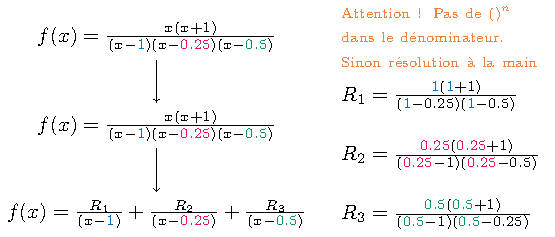
\includegraphics[width=7cm]{drwg_6.pdf}
\end{center}


\end{document}